\section{Proposed Measurements}
\label{sec:measurements}

The primary goal of the proposed experiment is to search for a heavy photon (dark photon) in the mass range from 20 MeV to 1000 MeV in at least two settings of beam energy 2.2 GeV and 6.6 GeV. 
HPS  ultimately relies upon the precision measurement of two quantities: the invariant mass of the A$^\prime$ decay products and the position of the decay vertex. By placing a tracking and vertexing detector immediately downstream of the target inside an analyzing magnet, the complete kinematic information required for A$^\prime$ reconstruction can be obtained from a single system, whose proximity to the target naturally maximizes the acceptance of a relatively compact detector and provides excellent momentum and vertexing resolution. A finely segmented, fast electromagnetic calorimeter, just downstream of the tracker,  provides a powerful high rate trigger, identifies electrons, and augments  the electron energy measurement. A muon system consisting of scintillator hodoscopes sandwiched between iron absorbers is also currently being considered as a potential upgrade. The muon system would provide a trigger for ($\mu^+\mu^-$) detection and  be used for muon identification. It would extend the search for high mass A$^\prime$ in di-muon decay mode. Very high rate data acquisition systems, for the tracker, Ecal and muon system, make it possible to trigger and transfer data at $10$s of kHz, and run with negligible dead time.

The HPS experiment also has the potential to discover ``true muonium'', a bound state of a $\mu^+ \mu^-$ pair and to search for non-minimal hidden sector final states.  

HPS plans to execute the full experiment in two phases. The first phase will start with a commissioning run in 2014 which will include data taking for roughly 2 weeks (on the floor) each at 1.1 and  2.2 GeV beam energies . More extensive data taking will continue in 2015, with runs at 2.2 and 6.6 GeV. This first phase will use about one sixth of the total beam time that HPS has requested, roughly 4 weeks on the floor at each of 2.2 and 6.6 GeV.  Assuming 50\% combined uptime for the accelerator and detector, this corresponds six weeks total of (perfect) run time:  1 week at 1.1 GeV, 3 weeks at 2.2 GeV, and 2 weeks at 6.6 GeV. The second phase of HPS running, which will occur in 2016 and beyond, will use the additional run time to extend the search for heavy photons to the largest possible region of parameter space, and study the properties of true muonium in detail.

\subsection{Search for the heavy photon}
\def \ap {A^\prime}
\def \map {m_{A^\prime}}
\def \thap {\theta_{A^\prime}}
%\subsubsection{Search for a Heavy Photon}
\label{sec:apsignal}




\begin{figure}
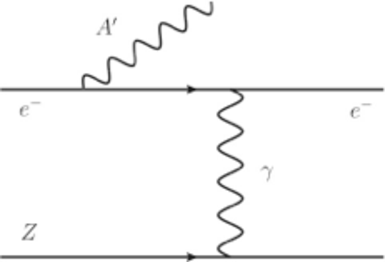
\includegraphics[scale=1]{measurements/Aprime-diagram.pdf}
\caption{Diagram of  $\ap$ production by bremsstrahlung off of an incoming electron scattering with an atomic nucleus.}
\label{fig:apdiagram}
\end{figure}

$\ap$ particles are generated in electron collisions on a fixed target by a process analogous to ordinary photon bremsstrahlung, see Figure \ref{fig:apdiagram}.  The rate and kinematics of $\ap$ radiation differ from massless bremsstrahlung in several important ways:
\begin{itemize}
\item  {\bf Rate}: The total $\ap$ production rate is controlled by $\alpha^3\epsilon^2 / m_{\ap}^2$.  
 Therefore, it is suppressed relative to photon bremsstrahlung by $\sim \epsilon^2 m_e^2/m_{\ap}^2$. 
\item {\bf Angle}:  $\ap$  is dominantly  emitted at  small angles ($\theta_{\ap}$).  Near its median value, the cutoff emission angle is
\begin{equation}
\theta_{\ap,max}\sim max\left(\frac{\sqrt{\map m_e}}{E_0},\left(\map/E_0\right)^{3/2}\right),
\end{equation}
which is parametrically smaller than the opening angle of the $\ap$ decay product, $\sim  \map/E_0$.  Although this opening angle is small, the backgrounds mimicking the signal dominate at even smaller angles.
\item {\bf Energy}:  $\ap$ bremsstrahlung is sharply peaked at $x=E_{A^\prime}/E_{beam}\approx 1$.  When an $\ap$ is produced, it carries nearly the entire beam energy.  In fact, the median value of (1-x) is $\sim {\rm max}\left(\frac{m_e}{\map},\frac{\map}{E_0}\right)$.  
\item{\bf Lifetime} For the ranges of $\epsilon$ and $\map$ probed by this experiment, the mean decay length $l_0$ of the $\ap$ can be prompt or as large as tens of centimeters.   The coupling and mass dependence is:
\begin{equation}
l_0 \equiv \gamma c\tau \approx \frac{0.8 cm}{N_{eff}} \left(\frac{E_0}{10 GeV}\right)\left(\frac{10^{-4}}{\epsilon}\right)^2\left(\frac{100 MeV}{\map}\right)^2.
\end{equation}
All of the background decays promptly at the target.  
\end{itemize}
The  latter three properties are quite important in resolving signal events from the main backgrounds, as discussed
below.   More details of $\ap$ production and decay are given in Appendix \ref{app:ProdAndDecay}.

The irreducible background rates are given by the diagrams shown in Figure \ref{fig:radbhdiagram}. These trident events can be usefully separated into "radiative" diagrams (Figure \ref{fig:radbhdiagram} (a)), and "Bethe-Heitler" diagrams (Figure \ref{fig:radbhdiagram} (b)), that are separately gauge-invariant.  These QED tridents dominate the final event sample, so we consider their properties in some detail here.

\begin{figure}
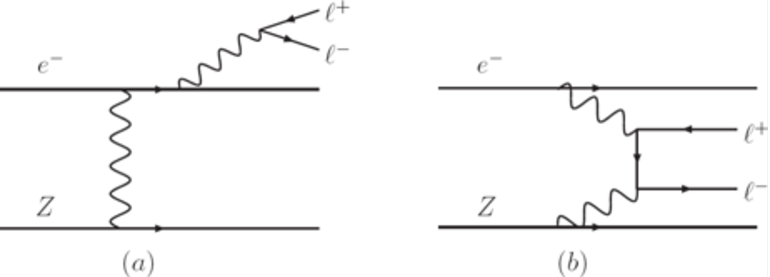
\includegraphics[scale=1]{measurements/rad-bh-diagrams.pdf}
\caption{Sample diagrams of (left) radiative trident ($\gamma^*$) and (right) Bethe-Heitler trident reactions that comprise the primary background to the $\ap\rarr l^+l^-$  search.}
\label{fig:radbhdiagram}
\end{figure}

The contribution from the radiative diagrams (Figure \ref{fig:radbhdiagram} (a)) alone is also useful as a guide to the behavior of $\ap$ signals at various masses. Indeed, the kinematics of the $A'$ signal events is identical to the distribution of radiative trident events restricted in an invariant mass window near the $A'$ mass. Moreover, the rate of the $A'$ signal is simply related to the radiative trident cross-section within the spectrometer acceptance and a mass window of width $\delta m$ by 
%\cite{4}
\begin{equation}
\frac{d\sigma\left(e^- Z \rarr e^- Z(\ap\rarr l^+l^-)\right)}{d\sigma\left(e^- Z \rarr e^- Z(\gamma^*\rarr l^+l^-)\right)}=\frac{3\pi\epsilon^2}{2 N_{eff}\alpha}\frac{\map}{\delta m}, 
\end{equation}
Where $N_{eff}$ is the number of final states that are open to the $A'$ to decay to.  This exact analytic formula was also checked with a MC simulation of both the $\ap$ signal and the radiative trident background restricted to a small mass window $\delta m$, and we find nearly perfect agreement. Thus, the radiative subsample can be used to analyze the signal, which simplifies the analysis considerably.

 Although the Bethe-Heitler process has a much larger total cross-section than either the signal or the radiative trident background, it can be significantly reduced by exploiting its very different kinematics. In particular, the $\ap$ carries most of the beam energy while the recoiling electron is very soft and scatters to a wide angle. In contrast, the Bethe-Heitler process is not enhanced at high pair energies. Moreover, Bethe-Heitler processes have a forward singularity that strongly favors asymmetric configurations with one energetic, forward electron or positron and the other constituent of the pair much softer.
These properties are discussed further in the Appendix of [4], and illustrated in Figure \ref{fig:tridentkinematics}.

\begin{figure}
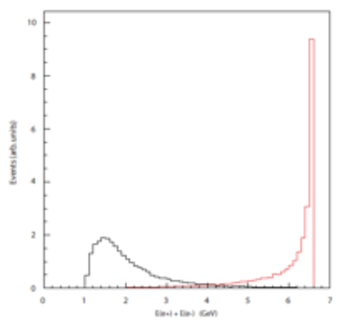
\includegraphics[scale=1.4]{measurements/rad-bh-energy.pdf}
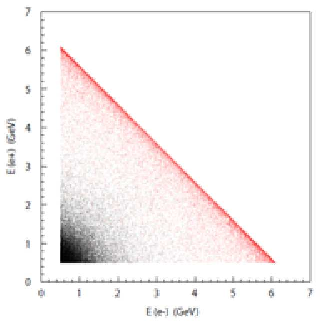
\includegraphics[scale=1.4]{measurements/E1vsE2.pdf}
\caption{ Left: The distribution of Bethe-Heitler background events (black) and radiative events (red) as a function of the sum of the electron and positron energy. Note that the radiative events  are peaked at high energies, while the Bethe-Heitler background is peaked at much lower energies. Right: The distribution of the positron versus electron energy for Bethe-Heitler  events (black dots) and radiative events (red dots). Note that in both plots the radiative and Bethe-Heitler events  are normalized to the same number. In reality, the number of Bethe-Heitler  events is much larger (prior to kinematic cuts) than the number of radiative events. After making a reasonable kinematic cut, the rates of Bethe-Heitler and radiative events are roughly the same.  Also, note that the electron energy here refers to the energy of the electron produced in the reaction, not the recoiling beam electron.}
\label{fig:tridentkinematics}
\end{figure}



\begin{figure}
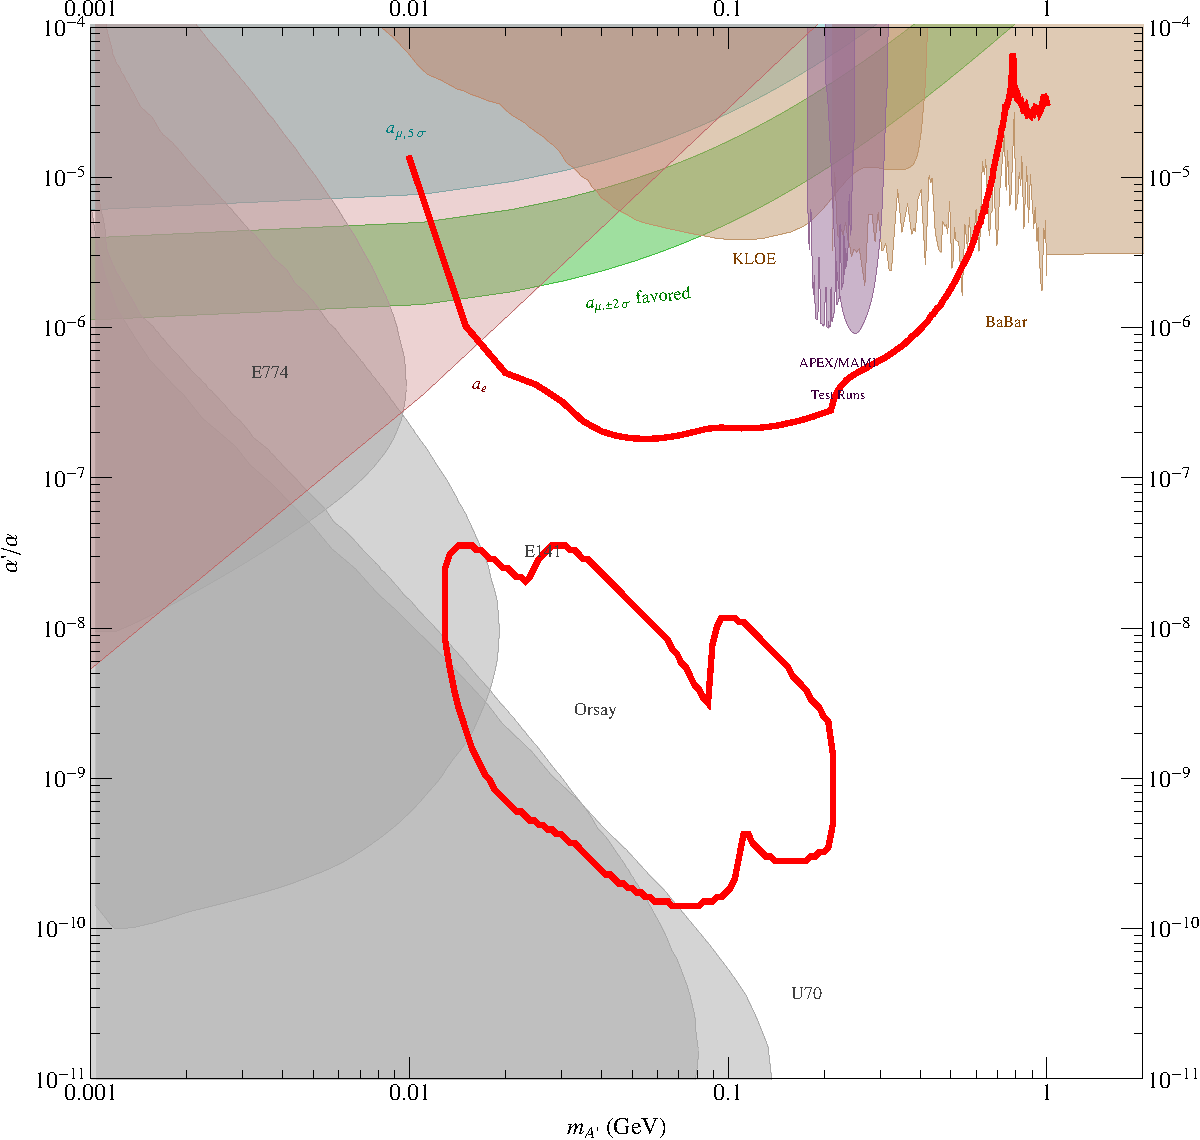
\includegraphics[width=0.9\textwidth]{measurements/HPS-Proposal2014-SimpleReach.pdf}
\caption{Expected mass vs coupling parameter space reach  full 2014-2015 running (solid red). Red line contour corresponds to 1 week of beam time at 1.1 GeV, and 3 weeks of beam time at 2.2 GeV and 6.6 GeV.}
\label{fig:reach}
\end{figure}

The radiative and Bethe-Heitler backgrounds show a smooth, continuous distribution in $m_{e^+e^-}$ and occur promptly at the production target.  The $A'$, however, will produce a peak at $m_{e^+e^-}=m_{A'}$ and, at lower values of $\epsilon$ have a vertex that is displaced from the target.  These two characteristics have led us to design a detector with both good momentum and spatial resolution.    The expected parameter reach in the first phase of the HPS is shown in Figure \ref{fig:reach}. The reach in mass-coupling parameter space is calculated using the simulated detector response as shown in Section \ref{sec:performance}.  The plot shows two distinct regions,  one at larger coupling corresponding to a purely bump-hunt region and another at lower coupling where the vertex of the $\ap$ decay is displaced.  



\subsection{Search for true muonium}

The proposed HPS experiment has the potential to discover ``true muonium'', a bound state of a
$\mu^+ \mu^-$ pair, denoted here by $(\mu^+ \mu^-)$. 
We expect that HPS will discover the 1S, 2S, and 2P true muonium bound states with its proposed run plan. 
The detection of these states should demonstrate the capability of the HPS experiment 
to identify rare separated vertex decays, and will provide a natural calibration 
tool for improving searches for heavy photons.
The $(\mu^+ \mu^-)$ atom is hydrogen-like, and so has a set of excited states characterized by a principal quantum number n. 
The binding energy of these states is E = $-1407$ eV/n$^2$. The $(\mu^+ \mu^-)$ ``atom'' can be produced by an electron beam incident on a target such 
as tungsten \cite{Holvik:1986ty,ArteagaRomero:2000yh}. 

With the existing proposal, HPS will search for true muonium
just as it does for heavy photons with separated vertices, requiring a vertex cut at about 1.5 cm to reject almost all
QED background events, then searching for a resonance at 2 m$_{\mu}$. An additional cut 
on the total energy of the $e^+e^-$ pair of $E_{e^-}+E_{e^+}> 0.8 \ E_{beam}$ will also be required
for triggering. 

Based on \cite{Banburski:2012tk}, the total production yield for 1S, 2S, and 2P (including secondary production)
leaving a target of thickness $t_b$(or larger) and satisfying the above requirements is,
\begin{equation}
N_{(\mu^+ \mu^-)} = 200 \left( \frac{I}{450 \ nA} \right) \left( \frac{t}{1 \ month} \right)\sim ~ 100 ~events 
\end{equation}
%
where a beam energy E$_{beam} = 6.6$ GeV, and the nominal conditions
of 450 nA beam current for 2 weeks of beam-time on a single foil has been assumed.
The vertices near the cut of $1.5$ cm will be dominated by the 1S state, while 
a tail of vertices extending out beyond a few cm is dominated by 2S and 2P. 

Accounting for all the efficiencies associated with a separated vertex search, we would expect to see about 10--20 true muonium events in 2 weeks of $6.6$ GeV run
(we caution that the acceptance parameterization here is uncertain at the 50\% level).
The HPS experiment should be able to identify enough events to claim a discovery, and in addition, should be able to measure the mass of true muonium.  There are certainly other properties of true muonium that would be interesting to measure.  A measurement of the lifetimes would be interesting, as the lifetimes are sensitive to physics that couples to leptonic currents.  With enough statistics, it should be possible to perform a measurement of the lifetimes of the 1S, 2S, and 2P states; work is ongoing to investigate this possibility.  

\subsection{Other searches for hidden sector particles}
\label{sec:hidden_ex}

While the primary motivation for the HPS experiment is a search for $\ap$ decaying to lepton pairs, following Arkani-Hamed {\it et al.\/}\cite{ArkaniHamed:2008qn}, it is useful to explore the sensitivity of HPS to other hidden sector particles, in particular those associated with Hidden Valley (HV) scenarios. As Strassler and Zurek\cite{Strassler:2006im} pointed out, HV scenarios provide many natural explanations of Dark Matter. The recent discovery of a boson that seems to have the properties of the Higgs boson of the Standard model also brings an old problem to the fore: why is the Higgs mass so light compare to the Planck scale? Searches at the LHC for supersymmetric partners and other particles with Standard Model couplings have so far been unsuccessful, pushing the range of allowed masses for such particles higher and higher. HPS may be the first in a series of experiments that complement the energy frontier searches by looking for new, light particles that couple to the SM particles through new, very weak forces. Just as one should be ready for the  unexpected when exploring the energy frontier at the LHC, so should we be in exploring the coupling frontier at with HPS.

In a general HV scenario, the new fermions may be lighter than the $\ap$ and have their own QCD-like forces, which results in them forming hidden mesons and baryons. Some of these hidden particles may be part of the Dark Matter. These hidden mesons would decay into SM fermion pairs  either democratically or with mass-dependent branchings. 
\begin{figure}[ht]
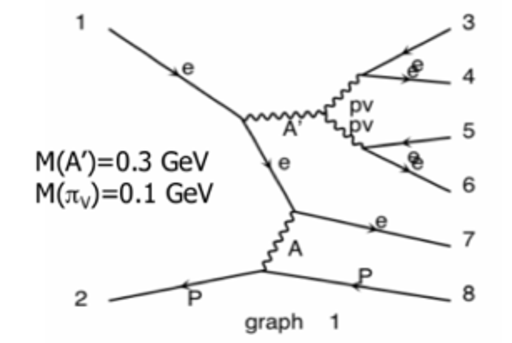
\includegraphics[scale=1]{measurements/multilepton-diagram.pdf}
\caption{Sample diagram of a non-Abelian hidden sector interaction.}
\label{fig:mldiagram}
\end{figure}
One interesting case is where the $\ap$ decays into a pair of dark mesons ($\pi_v$), which in turn promptly decay into electron pairs (see Fig \ref{fig:mldiagram}).  The high multiplicity of the typical final states makes an exclusive search for events such as these  difficult to trigger on, but it also reduces the background significantly by providing a number of new constraints and possible invariant mass bumps to search for and find.  Simulation studies are ongoing towards estimating the reach HPS has for such hidden mesons.  


%